\documentclass[final,onefignum,onetabnum]{siamart190516}
\usepackage[utf8]{inputenc}
\usepackage{geometry, graphicx,wrapfig}
\usepackage{enumerate}
\usepackage{amsmath,amssymb,amsfonts,bm}%,amsthm}
\usepackage{xcolor} %just for visible comments.
\usepackage[linesnumbered,ruled,vlined,algo2e]{algorithm2e}
\usepackage[toc,page]{appendix}
\usepackage{makecell}
\usepackage{cleveref}
\usepackage{pdfpages}

% New theorems and commands
\newtheorem{assump}[theorem]{MP Setting}
\newcommand\mycommfont[1]{\ttfamily\textcolor{orange}{#1}}
\newcommand{\R}{\mathbb{R}}
\newcommand{\F}{\mathbb{F}}
\newcommand{\dd}{\delta}
\newcommand{\tth}{\theta}
\newcommand{\bb}[1]{\mathbf{#1}}
\newcommand{\fl}{\mathrm{fl}}
\newcommand{\cO}{\mathcal{O}}
\newcommand{\red}[1]{\textcolor{red}{#1}}
\begin{document}
\title{Response to Reviewers}
\date{}
\maketitle
We are once again grateful to our editor, Laura Grigori, for handling the reviews of our paper, and to both reviewers for their constructive criticisms.

Our response to the reviews is below and the appropriate changes are shown below. We have not appended a diff file this time.\\

\noindent{\bf Reviewer \#1}
\begin{enumerate}
	\item \textit{line 548-549 (in diff): I would reword this sentence, which implies that here TSQR is guaranteed high accuracy in this scenario. In fact, the found is ~1e-2, which I don't think qualifies as ``high accuracy''.}\\
	\textbf{Original sentence:} This case exemplifies a situation in which high accuracy is not guaranteed in HQR, but it is guaranteed when using TSQR.\\
	\textbf{New sentence:} ``This case exemplifies a situation in which accuracy is not guaranteed in HQR, but a relative error of $\approx 3.5\%$ is guaranteed when using TSQR. ''
	\item \textit{The font on the axes labels in Figure 3 (two rightmost plots) should be made larger.}\\
	\textbf{The new figure is shown below.}
	\begin{figure}[h!]%{r}{.53\textwidth}
		\centering
		%\vspace{-10pt}
		\includegraphics[width=\textwidth]{../figures/allTSQR4.png}
		\vspace{-15pt}
		\caption{\label{fig:allTSQR} All plots show the backward relative error for 4000-by-100 sized test matrices. Left: {\tt mpHQR2} on condition numbers ranging from 1.1 to 101;  Middle: {\tt mpTSQR2} on condition numbers ranging from 5.3 to 101; Right:  {\tt mpTSQR2} on condition numbers ranging from 1.1 to 5.3.  The red line on both plots corresponds to value {\tt 5.2e-3},and the green/blue segments show a decrease/increase in error in comparison to using TSQR with one fewer level. }
		\vspace{-5pt}
	\end{figure}
	
\end{enumerate}

%\bibliographystyle{siamplain}%ieeetr
%\bibliography{../../../../../library.bib,../../../../../sans_library.bib,./report.bib}

%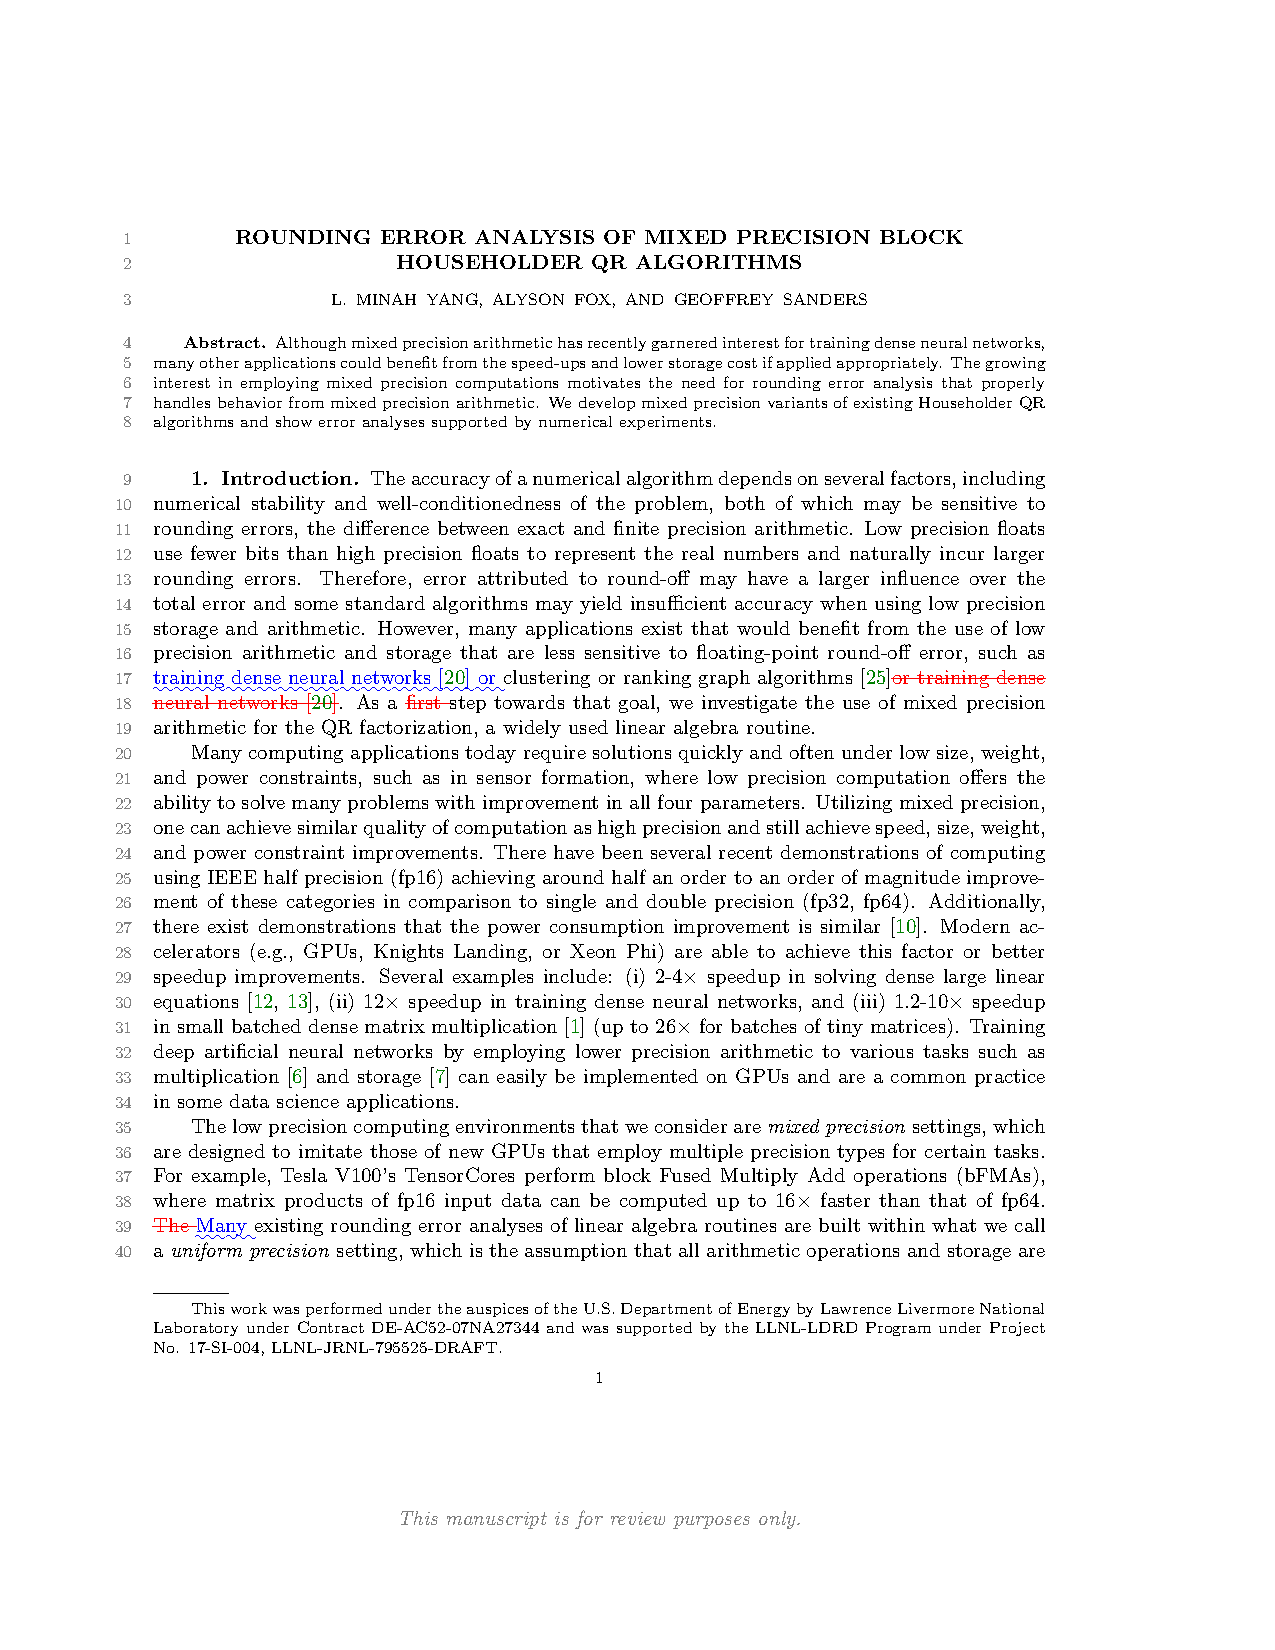
\includepdf[pages=-]{diff0105.pdf}
\end{document}